\documentclass[12pt]{article}
\usepackage[utf8]{inputenc}
\usepackage{longtable}
\usepackage{multirow}
\usepackage{graphicx}
\graphicspath{ {./author/} }
\renewcommand{\baselinestretch}{1.5}


\title{John von Neumann(1903-1957)}
\author{Luis Diego Jiménez Delgado}
\date{Agosto 12 del 2019}

\begin{document}

\maketitle
\begin{center}
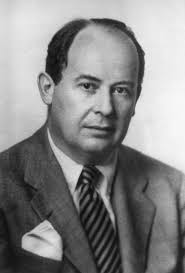
\includegraphics{na}
\end{center}
John von Neumann fue un matemático húngaro-estadounidense que realizó contribuciones fundamentales en física cuántica, análisis funcional, teoría de conjuntos, teoría de juegos, ciencias de la computación, economía, análisis numérico, cibernética, hidrodinámica, estadística y muchos otros campos. Se le considera uno de los matemáticos más importantes del siglo XX.
\end{document}